\section{Figures Instagram}

\begin{figure}[!htb]
	\centering
	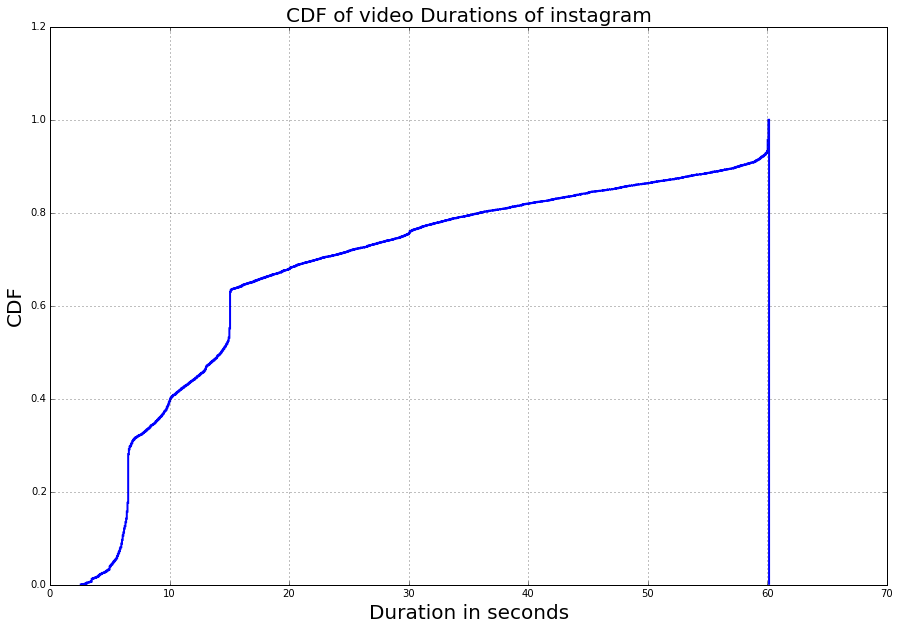
\includegraphics[width=\columnwidth]{plots/VideoDurationInsta.png}
	\caption{\textsl{CDF of instagram video lengths across the complete 15k videos. The figure shows that despite relaxed time constraint, 70\% of the videos are smaller than 20 seconds long}}
	\label{fig:Face_Thirds}
\end{figure}


\begin{figure}[!htb]
	\centering
	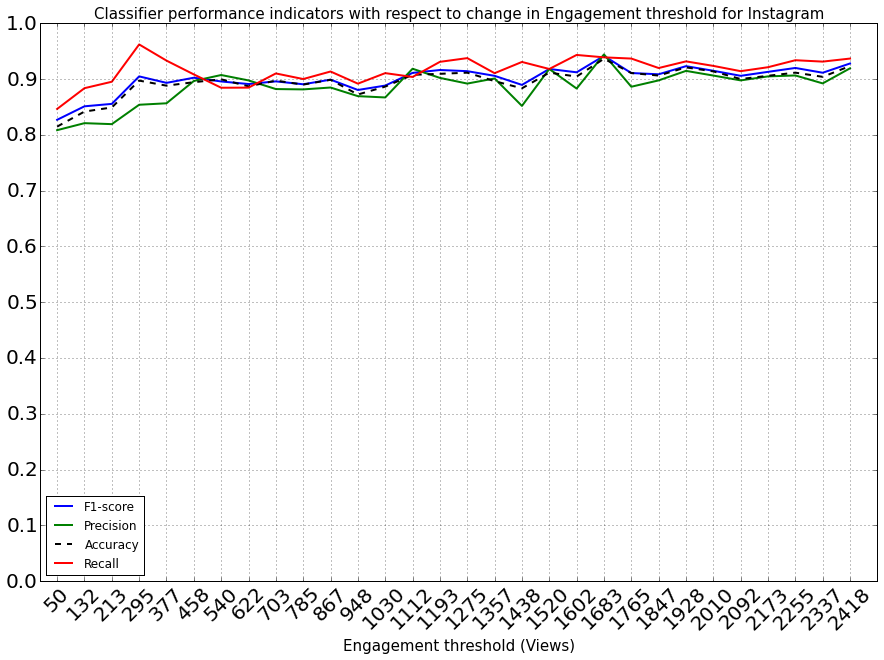
\includegraphics[width=\columnwidth]{plots/InstaClassifierPerf.png}
	\caption{\textsl{SVM classifier performance. The classifier is trained using the exact same methodology as for Vine}}
	\label{fig:Face_Thirds}
\end{figure}


\begin{figure}[!htb]
	\centering
	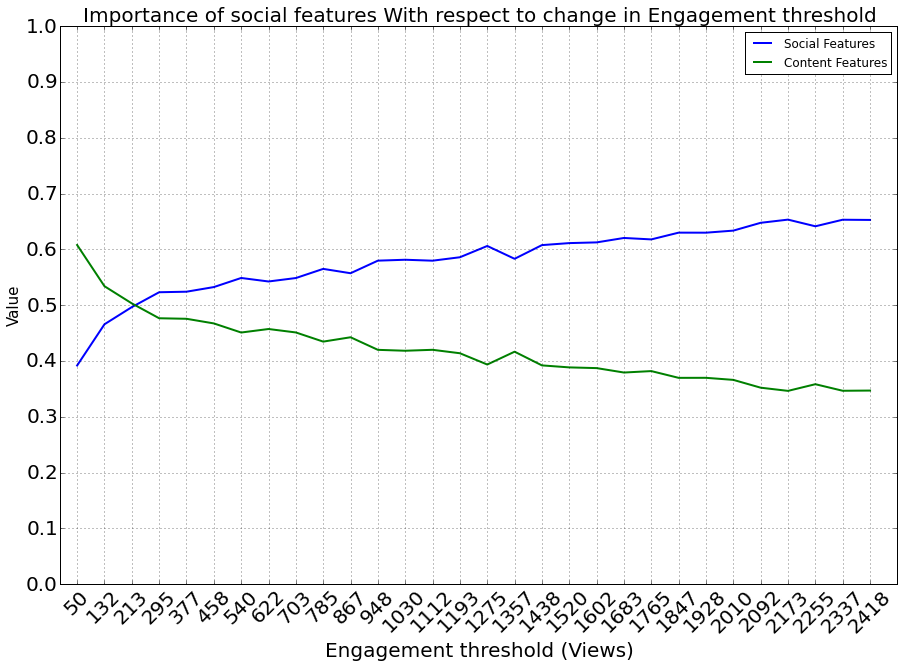
\includegraphics[width=\columnwidth]{plots/InstaSocialVsContent.png}
	\caption{\textsl{Social Vs Content feature importance for Instagram videos. There is a contradictory phenomenon here compared to Vine. This is because in case of Instagram the content features play a major role in till you get into the top 25 percentile of engagement, but then the social features become more important  }}
	\label{fig:Face_Thirds}
\end{figure}

\begin{figure}[!htb]
	\centering
	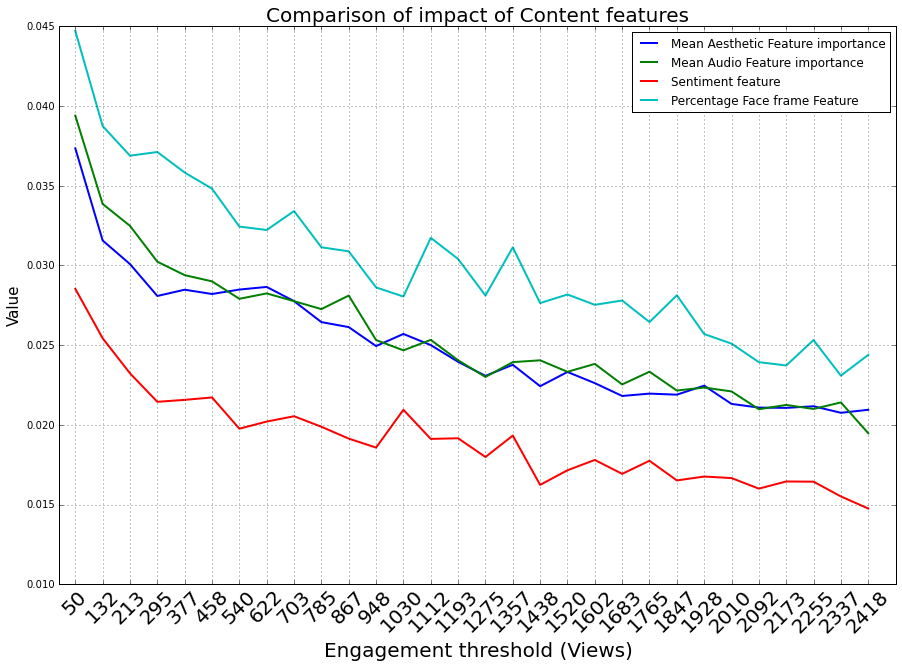
\includegraphics[width=\columnwidth]{plots/InstaContentComparison.png}
	\caption{\textsl{Content Feature importance variation for the Instagram classifier }}
	\label{fig:Face_Thirds}
\end{figure}

\begin{figure}[!htb]
	\centering
	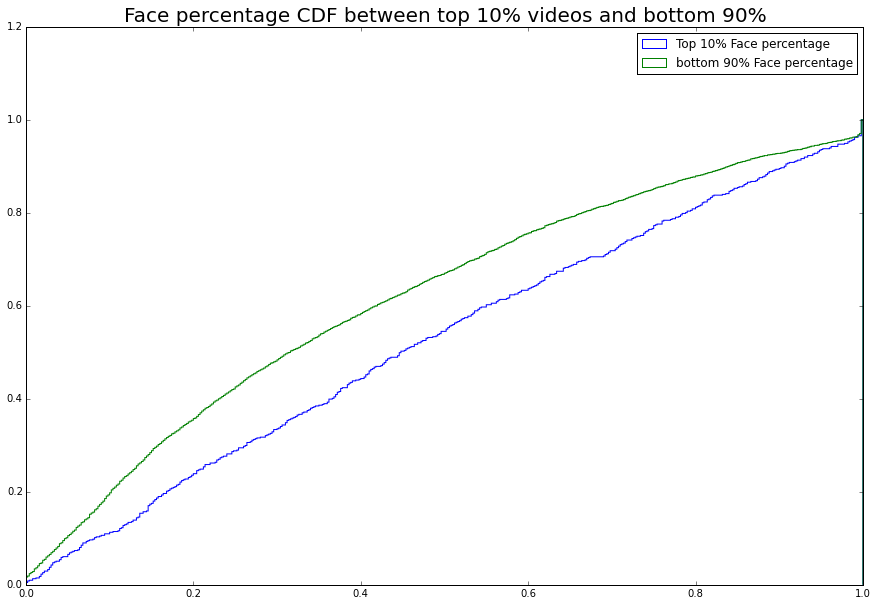
\includegraphics[width=\columnwidth]{plots/FacepercentageInsta.png}
	\caption{\textsl{Social features (followers , followed) feature importance}}
	\label{fig:Face_Thirds}
\end{figure}